\section{Analýza}
\subsection{Operačné systémy}
\indent Informatika a informačné technológie je pomerne mladá vedná disciplína. Jej začiatky je možné datovať od druhej polovice dvadsiateho storočia, čo momentálne predstavuje takmer sedemdesiat rokov. Za tento čas informatika zaznamenala enormný rast vo vývoji hardvéru, ako aj softvéru.  Operačný systém je základná časť akéhokoľvek počítačového sytému, predstavuje softvér, ktorý umožňuje počítačom pracovať. V poslednej dobe, oblasť operačných systémov  prechádza rapídnymi zmenami, pretože počítače sa stali súčasťou každodenného života, a to od malých zariadení, napríklad v automobiloch, až po najsofisitkovanejšie servery nadnárodných spoločností. Aj napriek tomu, že v dnešnej dobe poznáme mnohé operačné systémy, v práci sa zameriame na Windows, Mac OS, Unix a Linux.\cite{osbook}

\subsubsection{Windows}
\indent Microsoft Windows uviedol svoje prvé operačné systémy v novembri roku 1985 ako nadstavbu MS DOS. Jeho popularita rýchlo rástla až vyvrcholila dominantným postavením na trhu v osobných počítačoch. V roku 1993 začal vydávať špecializované operačné systémy, ktoré prinášali novú funkcionalitu pre počítače používané ako servery.\cite{windowsHistory} Pre účely automatizácie sa na Windows serveroch používajú hlavne powershell scripty, písané v rovnomennom jazyku Powershell\cite{winAutomation}.
\paragraph{Podiel na trhu}
\indent Microsoft je aj vzhľadom na svoju históriu najobľúbenejším operačným systémom v segmente osobných počítačov. Podľa webovej stránky statcounter.com\cite{statcounter} a netmarketshare.com\cite{netmarketshare} má 81,73\%  \gls{resp.}  88,42\% podiel na trhu.
\newline
\indent Podľa w3techs.com\cite{pop} je serverový operačný systém Windows používaný na 32.0\% počítačoch.
\paragraph{Predinštalovaný softvér}
\indent Windows operačné systémy ponúkajú základný balík nástrojov a programov. Serverové aj neserverové verzie Windowsu ponúkajú  Powershell, ktorý je dostupný od inštalácie.  Oba systémy podporujú aj takzvaný Command prompt alebo príkazový riadok, ktorý je alternatívou k Powershellu. Akékoľvek ďalšie programy je potrebné stiahnuť a doinštalovať.

\subsubsection{MacOs}
\indent  Mac okrem iného ponúka serverovú verziu operačného systému pod názvom OS X Server, ktorý začal písať svoju históriu v roku 2001, avšak neteší sa takej obľube ako Windows, Unix alebo Linux server. OS X server nepoužíva  špecifický skriptovací jazyk, pričom poskytuje možnosť výberu skriptovacieho jazyka, ako napríklad: Python, JavaScript, Perl, AppleScript, Swift alebo Ruby. Každý z uvedených jazykov prináša určité plusy, ako aj mínusy.
\paragraph{Predinštalovaný softvér}
\indent Predinštalovaný softvér pre developerov na Mac OS je Python, AppleScript, Ruby, Bash, BOjective-c. Donedávna bola štandardom aj Java, avšak Apple sa rozhodol pre radikálny krok vylúčiť Javu a propagovať Objective-c.
\paragraph{Podiel na trhu}
\indent Popularita počítačov s predinštalovaným operačným systémom MacOs sa mierne zvyšuje, čo je možné vidieť aj na obrázku na konci sekcie operačných systémov. Podľa webovej stránky statcounter.com\cite{statcounter} a netmarketshare.com\cite{netmarketshare} mu patrí 13,18\% resp.  9,19\% na trhu.
\indent Serverové verzie MacOs podľa stránky w3techs.com\cite{pop} sú na menej ako 0.1\% zariadeniach.
\subsubsection{Unix}
\indent Patrí medzi prvé operačné systémy pre servery, ktorého vývoj začal v roku 1970 a v priebehu rokov vzniklo veľa nových verzií Unixu a Linuxu. V minulosti boli Unixové servery veľmi obľúbené, avšak v súčasnosti sú na ústupe, a to najmä kvôli vyšším obstarávacím a prevádzkovým nákladom. Pre účely Unixu sa vytvoril Unix shell, dostupný v rôznych obmenách, ktorý je často vyhľadávaným jazykom medzi administrátormi a automatizačnými programátormi.
\paragraph{Predinštalovaný softvér}
\indent Na vačšine unixových systémoch je predinštalovaný Shell a Open JDK.
\paragraph{Podiel na trhu}
\indent Podľa stránky w3techs.com\cite{pop} sa Unixové systémy používajú na rovných 68.0\% počítačov.
\subsubsection{Linux}
\indent  Linux je všeobecný názov pre širokú zostavu Linux distribúcií, ktoré používajú Linux Kernel. Linux Kernel bol prvýkrát verejnosti predstavený v roku 1991 a odvtedy bol rozšírený na najviac platforiem. Momentálne je jediným používaným operačným systémom na TOP 500 superpočítačoch (mainframe). Skriptovacím jazykom pre Linux je Unix Shell resp. jeho najrozšírenejšia forma Bash.
\paragraph{Predinštalovaný softvér}
\indent Predinštalovaný softvér vo väčšine distribúciách Linuxu sú Bash, Open JDK - Java, niektoré distribúcie ponúkajú Python. RedHat začína s podporou .net frameworku.
\paragraph{Podiel na trhu}
\indent Linux je k dispozícii v mnohých formách, tak aby vyhovoval rôznym potrebám, od spotrebiteľsky orientovaných systémov pre domáce použitie až po distribúcie použiteľné v špecifických odvetviach. Podľa webovej stránky statcounter.com\cite{statcounter} a netmarketshare.com\cite{netmarketshare} mu patrí 1,66\% resp.  1,93\%.
Podľa stránky w3techs.com\cite{pop} je operačný systém Linux na 41.0\% počítačoch.
\subsubsection{Grafy}
\indent Nasledujúce grafy zobrazujú podiel operačných systémov na trhu v segmente osobných počítačov, ako aj v segmente serverov. Zaujímavý graf je vývoj trendu využívania serverových operačných systémov, z ktorého vidíme, že unixové a linuxové servery zvyšujú svoje podiely na trhu. Naopak, Windows v posledných mesiacoch stratil pár percent. Taktiež je vidieť, že linuxové a unixové systémy pokrývajú viac ako polovicu web stránok, ktoré majú najvyššie hodnotenie.
\begin{figure}[!htbp]
	\centering
	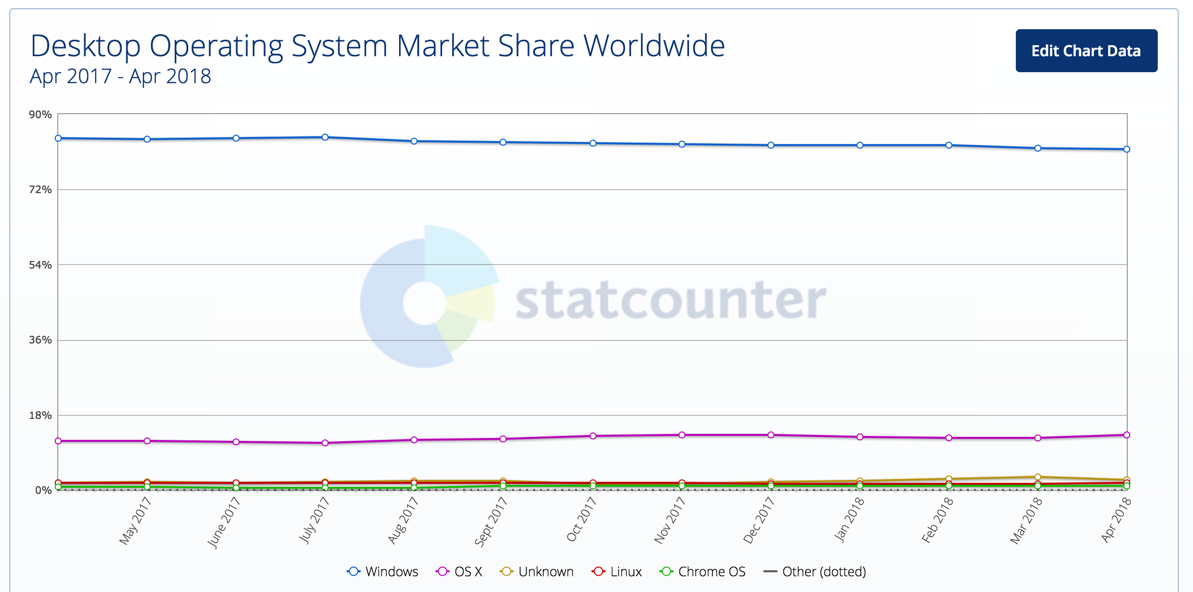
\includegraphics[width=\linewidth]{img/statcounter.png}
	\caption{\gls{os} - podiel na trhu podľa statcounter\cite{statcounter}}
	\label{fig:test}
	
\end{figure}
\begin{figure}[!htbp]
	\centering
	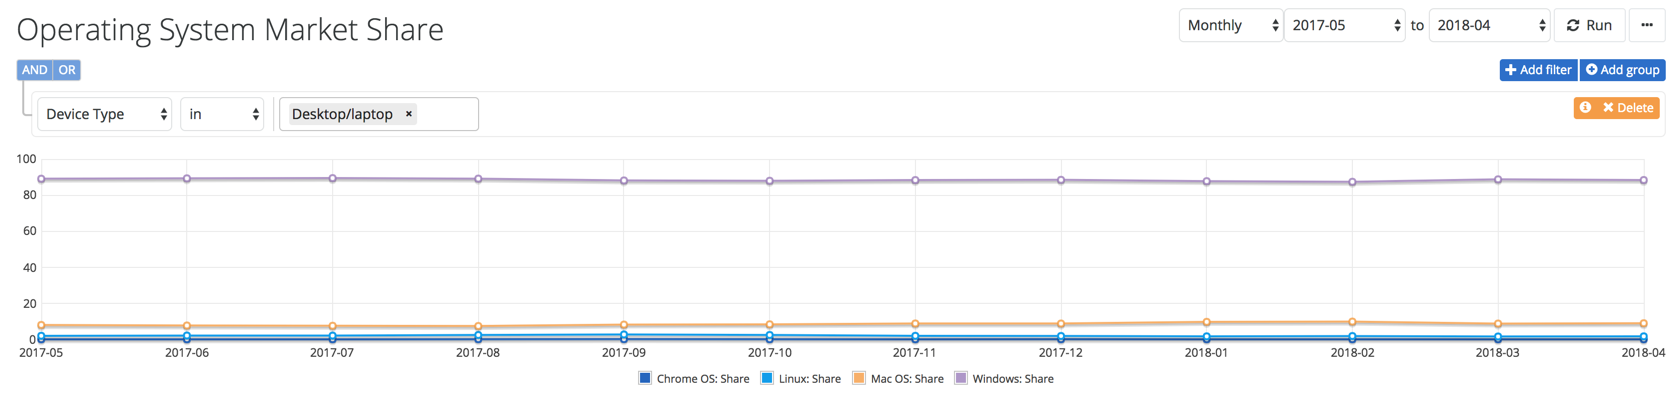
\includegraphics[width=\linewidth]{img/netmarketshare.png}
	\caption{\gls{os} - podiel na trhu podľa netmarketshare\cite{netmarketshare}}
	\label{fig:test}
	
\end{figure}
\begin{figure}[!htbp]
	\centering
	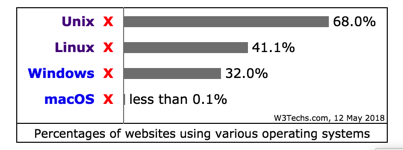
\includegraphics[scale=0.4]{img/usg_server.png}
	\caption{Serverové \gls{os} - podiel na trhu podľa w3techs\cite{pop}}
	\label{fig:test}
	
\end{figure}
\begin{figure}[!htbp]
	\centering
	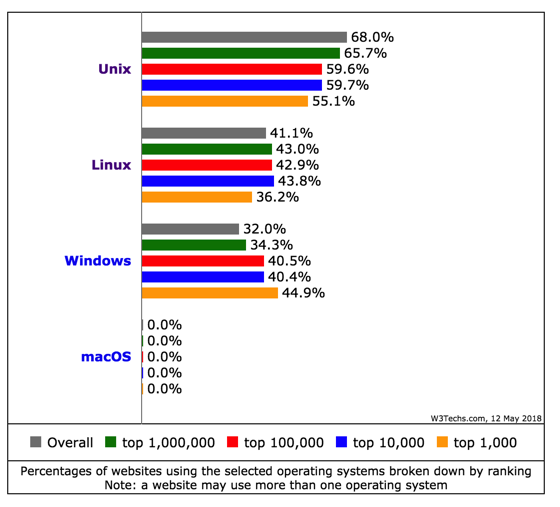
\includegraphics[scale=0.4]{img/usage_grou_by_os_sites.png}
	\caption{Serverové \gls{os} - podiel na trhu a rozdelenie podľa hodnotenia stránok podľa w3techs\cite{pop}}
	\label{fig:test}
	
\end{figure}

\subsection{Programovacie jazyky}
\indent S príchodom osobných počítačov no najmä serverov, sa programátori zaujímali o automatizáciu procesov, ktoré na danom stoji bolo spočiatku potrebné spúšťať manuálne. Nakoľko tieto úlohy neboli na toľko komplexné ako samotné programy, ktoré spúštali bolo vhodné na tieto úlohy využiť/vytvoriť skriptovacie jazyky. V nasledujúcej časti si priblížime zopár programovacích jazykov, ktoré sa v dnešnej dobe bežne používajú na tvorbu automatizovaných skriptov.

\subsubsection{Shell}
\indent
Je skriptovacím jazykom pre unixové distribúcie. Počas rokov prešiel roznymi zmenami a rozšíreniami. Verzie shellu su: sh, csh, ksh,tcsh, bash. Bash sa momentálne teši najväčšej obľube no zsh je verzia shellu, ktorá má najviac rôznych rozšírení funkcionality ako aj veľa priaznivcov medzi developermi. V nasledujúcich častiach všeobecne zhodnotíme jednotlivé výhody resp. nevýhody tohoto skriptovacieho jazyka.

\paragraph{Výhody}
\begin{itemize}
	\item automatizácia často opakujúcich sa úloh
	\item dokáže zbiehať zloťité zloťené príkazy ako jednoriadkový príkaz  - tzv. reťazenie príkazov
	\item ľahký na používanie
	\item výborné manuálové stránky
	\item ak hovoríme o Unix shelli je portabilný naprieč platformami linuxu-unixu
	\item jednoduché plánovanie automatických úloh
	\newline
\end{itemize}
\paragraph{Nevýhody}
\begin{itemize}
	\item asi najväčšou nevýhodou je ze natívne nefunguje pod windowsom, existuju iba rozne emulátory a nástroje tretích strán, ktoré sprostredkujú jeho funkcionalitu.
	\item pomalé vykonávanie príkazov pri porovnaní s inými programovacími jazykmi
	\item nový proces pre skoro každý spustený príkaz
	\item zložitejší na pamatanie si rôznych prepínačov, ktoré dané príkazy podporujú
	\item nejednotnosť prepínočov(hoc to by asi ani nešlo)
	\item neprenosný medzi platformami
	\item shell nepridáva vlastné príkazy, používa iba tie, ktoré sú dostupné na konkrétnom počítači
\end{itemize}
\paragraph{Popis a zhodnotenie jazyka}
\indent
Unix Shell je obľúbeným scriptovacím jazykom, vhodným na automatizovanie každodenných operácií. Je jedným z najpoužívanejších skriptovacích jazykou vôbec, nakoľko všetky linuxove, unixové servery využívajú práve tento jazyk ako svoj primárny. V nasledujujucich častiach budem popisovať Bash, ktorý je najrozšírenejšia verzia Unix shellu. Medzi jeho silné stránky patrí jednoduchá manipulácia s crontable, pomocou ktorej vie admin jednoducho planovať beh procesov. Ďalšou zaujímavou vymoženosťou jazyka je pajpa. Pajpa je klasickým príkladom vnútro-procesorovej komunikácie : odovzdáva štandardný výstup "stdout" procesu na štandardný vstup "stdin"iného procesu, viď príklad.
\begin{minted}[]{php}
	zarrelli:~\$ ls -lah | wc -l
	35
\end{minted}
V uvedenom príklade sme vylistovali obsah adresára v ktorom sa práve nachádzame a výstupom z programu sme naplnili štandardný vstup aplikácie "wc" ktorá spočíta, koľko riadkov sa nachádza vo vstupe, ktorý jej bol dodaný. Príkaz za znakom pajpy "|" beží v subshelli, čo znamená, že nebude schopný zmodifikované hodnoty v rodičovskom procese. Zlyhanie príkazu v pajpe vedie k takzvanej "zlomenej pajpe", v tomto prípade exekúcia príkazov skončí. \cite{mbash}
\newpage
Taktiež niektoré často používané príkazy majú pozmenený spôsob zápisu.
Ako príklad si uvedieme príkaz for, pri ktorom bash používa nsledovnú syntax:

\begin{algorithm}
	\begin{minted}{php}
// prvý spôsob zápisu podobná vylepšenej verzii z predchádzajúceho príkladu
for placeholder in list_of_items
do
action_1 \$placeholder
action_2 \$placeholder
action_n \$placeholder
done
//kolekcia vo fore môze byť reprezentovaná vymenovaním prvkov 
//priamo za "in" časťou
for i in 1 2 3 4 5
do
echo "\$i"
done
// c-like prístup
for ((i=20;i > 0;i--))
{
	if (( i % 2 == 0 ))
	then
	echo "\$i is divisible by 2"fi
}
exit 0
	\end{minted} 
	\caption{Bash ukážka rôznych volaní for cyklu. \cite{mbash}}
\label{alg:gen}
\end{algorithm}

Ako je vidieť z príkladu for používa podobnú syntax ako ostatné jazyky, a ešte ju rozširuje, druhý spôsob môže uľahčiť prácu napríklad pri prototypovaní skriptu. Vyššie spomenuté použitia niesú jediné, shell poskytuje možnosť vložiť parametre pre nasledovnú iteráciu priamo z konzoly ako v nasledovnom príklade.
\newpage
\begin{algorithm}
	\begin{minted}{php}
//telo skriptu
#!/bin/bash
i=0
for cities 
do
echo "City $((i++)) is: $cities"
done
exit 0

//následné volanie z konzoly
./for-pair-input.sh 
Belfast Redwood Milan Paris
City 0 is: Belfast
City 1 is: Redwood
City 2 is: Milan
City 3 is: Paris
	\end{minted}
	\caption{Bash ukážka volania skriptu s for cylom priamo z konzoly . \cite{mbash}}
	\label{alg:gen}
\end{algorithm}

Avšak syntax jazyka sa učí tažšie nakoľko používa rôzne prepínače, ktoré novému používateľovi nemusia byť sprvu jasné. 
V tabuľke uvádzame príklad prepínačov pre if, ktorý pre podmienkovú časť používa hranaté zátvorky namiesto okrúhlych na aké sme zvyknutý z väčšiny programovacích jazykov. Za zmienku stojí tiež, že napríklad Unix shell nepoužíva žiadne zátvorky v podmienkovej časti príkazu, na ukončenie podmienkovej časti sa používa bodkočiarka, čo spôsobuje problémi pri prenositeľnosti. If ponúka aj ďalšie prepínače no zhodnotili sme, že pre ilustráciu budú postačovať aj príklady uveené v tabuľke.
Najvačsia nevýhoda je, že ani shell script nieje jazyk, ktorý by bol multiplatformový a teda ak by sme mali prostredie, kde servery bežia na rôznych operačných systémoch, potrebujeme poznať ďalší jazyk, ktorým docielime rovnaké alebo aspoň podobné výsledky.
\newline
\begin{table}[h!]
	\centering
	\begin{tabular}{|p{4cm}|p{13cm}|}
		\hline
		Reťazcové porovnanie & Popis \\
		\hline
		Str1 = Str2	& Vráti true ak sa porovnávané reťazce rovnajú. \\ 
		\hline
		Str1 != Str2 &	Vráti true ak porovnávané reťazce nie sú rovnaké.\\ 
		\hline
		-n Str1	 &R Vráti true ak reťazec nie je null resp. o dĺžke 0.\\ 
		\hline
		-z Str1	& Returns true ak reťazec je null resp. o dĺžke 0.\\
		\hline
	\end{tabular}
\caption{Ukážka reťazcových prepínačov v podmienkovom výraze if \cite{shellprep}}
\label{table:1}

\end{table}
		\begin{table}[h!]
			\centering
			\begin{tabular}{|p{4cm}|p{13cm}|}
		\hline
		Numerické porovnanie	& Popis \\
		\hline
		expr1 -eq expr2	& Vráti true ak sú porovnávané výrazy rovné. \\
		\hline
		expr1 -ne expr2	& Vráti true if ak nie sú porovnávané výrazy rovné. \\
		\hline
		expr1 -gt expr2	& Vráti true ak je hodnota premmenej expr1 väčšia než hodnota premennej expr2. \\
		\hline
		expr1 -ge expr2	& Vráti true ak je hodnota premmenej expr1 väčšia alebo rovná hodnote premennej expr2. \\
		\hline
		expr1 -lt expr2	& Vráti true ak je hodnota premmenej expr1 menšia než hodnota premennej  expr2. \\
		\hline
		expr1 -le expr2	& Vráti true ak je hodnota premmenej expr1 menšia alebo rovná hodnote premennej expr2. \\
		\hline
		! expr1	& Operátor "!" zneguje hodnotu premennej expr1. \\
		\hline
	\end{tabular}
	\caption{Ukážka numerických prepínačov v podmienkovom výraze if \cite{shellprep}}
	\label{table:1}
	
\end{table}
\newpage

\subsubsection{Powershel/Classic command line}
\indent  
Command line je zakladnym skriptovacim jazykom pre windows distribucie, ktorý poskytuje malé API  pre svojich používateľov. Aj kôli tomu Miscrosoft prišiel s novým jazykom Powershell. Powershell je kombináciou príkazového riadku, funkcionálneho programovania a objektovo orentovaného programovania. Je založený na .NET frameworku, ktorý mu dáva istú mieru flexibility, ktorá v 

TODO: dpoisat dake sprostosti

Jeho vyhody a nevyhody si popiseme v nasledujujucich castiach.

\paragraph{Výhody}
\begin{itemize}
	\item bohaté api
	\item výborne riešeny run-time 
	\item flexibilný
	\item veľmi jednoduché prepnúť z .NET frameworku
	\item dokáže pridávať funkcionalitu používaním tired a funkcií z .net knižníc
	\newline 
\end{itemize}
\paragraph{Nevýhody}
\begin{itemize}
	\item bohaté api - nejednoznačné, kedy čo použiť
	\item niektoré výhody jazyka sú až nevhodne skryté pred používateľmi
	\item staršie verzie serverov nie sú Powershell-om podporované ako novšie
	\item dokumentácia je horšia ako v prípade Shell scriptu
	\newline
\end{itemize}

\paragraph{Popis a zhodnotenie jazyka}
Powershell je obľúbený medzi programátormi a administrátormi, ktorý pracujú pod operačným systémom Windowsu. Do nedávna kým Pewrshell bežal na .NET frameworku ho nebolo možné používať mimo operačných systémov Windows, avšak s príchodom frameworku .NET Core sa situácia zmenila. Tento frawework je momentálne open source, jeho zdrojové kódy boli zverejnené a je doň možné prispievať. Okrem iného podporuje rovnaké alebo aspoň podobné štruktúry ako Shell script a poskytuje v niektorých prípadoch rovnaké príkazy ako napríklad : mv, cp, rm, ls. Jednen zo zásadných rozdielov medzi Shellom a Powrshellom je ten, že kým v Shelli sú pre vstup aj výstup používané textové reťazce, ktoré je potrebné rozparsovať a interpretovať v Powershelli je všetko presúvané ako objekt. Po preštudovaní si materiálov jazyka z Mastering Windows PowerShell Scripting - Second Edition \cite{psbook}, ide o najzásadnejší rozdiel, nakoľko ostatné veci boli zrejme navrhované v spolupráci s používateľmi Shell scriptu.

Pre demonštráciu rozdielov pri odovzdávaní si parametrov medzi príkazmi prikladám nasledovný príklad.
\newpage
\begin{algorithm}
	\begin{minted}[]{php}
	function changeName(\$myObject)
	{
		if (\$myObject.GetType() -eq [MyType])
		{
			//vypíš obsah premennej
			\$myObject.Name
			//zmeň reťazec pre atribút name
			\$myObject.Name = "NewName"
		}
		return \$myObject
	}
	
	// Vytvorenie objektu s argumentom OriginalName a následné použitie funkcie na zmenu argumentu
	//PS> \$myObject = New-Object MyType -arg "OriginalName"
	//PS> \$myObject = changeName \$myNewObject
	//OriginalName
	//PS> \$myObject.Name
	//NewName
	// Ukážka s využitím pipe
	//PS> \$myObject = New-Object MyType -arg "OriginalName" | changeName
	//OriginalName
	//PS> \$myObject.Name
	//NewName
	\end{minted}
	\caption{Ukážka použitia pipe v powershell. \cite{netalg}}
	\label{alg:gen}
\end{algorithm}

\subsubsection{Python}
\indent Do analýzy sme sa rozhodli pripojiť aj Python. Python sme si nevybrali náhodne, nakoľko je jedným z najpopulárnejších programovacích jazykov súčastnosti. Je viacúčelový, patrí mezi vyššie programovacie jazyky, objektovo orientovaný, interaktívny, interpretovaný a extrémne používateľsky prijateľný.\cite{python}
\paragraph{Výhody}
\begin{itemize}
	\item Je ľahko čitateľný, tým pádom ľahšie pochopiteľný
	\item Syntax orientovaná na produktivitu
	\item Multiplatformový - po inštalácii interpretera
	\item Množstvo rôznych knižníc
	\item Open source
	\newline
\end{itemize}
\paragraph{Nevýhody}
\begin{itemize}
	\item Rýchlosť
	\item Slabšia dokumentácia
	\item Nevhodný pre úlohy pracujúce s vyšším množstvom pamäte
	\item Nevhodný pre viac-procesorovú prácu
	\item Nevhodný pre vývoj na mobilných zariadeniach
	\item Limitácie pri prístupe k databázam 
	\newline
\end{itemize}

\paragraph{Popis a zhodnotenie jazyka}
\indent Ako sme spomínali Python je jeden z najobľúbenejších jazykov súčastnosti, veľkú časť tejto komunity tvoria vedci, ktorý nemajú rozsiahle programátorské znalosti. Práve jednoduchosť, čitateľnosť a pochopiteľnosť jazyka sa nemalou mierou podieľajú na tomto fakte. Taktiež tu nieje nutné manažovať pamäť a iné netriviálne záležitosti ničších programovacích jazykov. Jazyk je síce objektovo orientovaný no jednoducho sa v ňom píšu aj skripty.  Jazyk poskytuje štruktúry ako pipa, dokážeme v ňom jednoducho pracovať s procesmi, vytvárať triedy, inštancie, jednoducho prototypovať a odsymulovať rôzne problémy. Veľkou výhodou tohoto jazyka je, že je open source s veľkou komunitou, ktorá rada testuje nové vydania, nahlasujú problímy a tým pádom sa jazyk rýchlejšie a kvalitnejšie vyvíja. Na Pythone vznikli zaujímave webové framworky ako napríklad Django. Každá strana má dve mince a ani Python nie je stopercentný. Tým, že je to interpretovaný jazyk neprekypuje rýchlosťou. Veľa ľudí sa zaoberá rýchlosťou jazykov, zisťujú efektívnosť pri rôznych úkonoch ako napríklad cykly, volania funkcií, aritmetika, prístup k pamäti, vytváranie objektov. V nasledujúcich tabuľkách je vidno rozdiel v rýchlosti jednotlivých testov. 
\begin{center}
	\begin{table}[htbp]
		\begin{tabular}{|p{2.5cm}|p{2.5cm}|p{2.5cm}|p{2.5cm}|}
			\hline
			\textbf{Jazyk} & \textbf{Force field benchmark}  & \textbf{Array reverse benchmark}&\textbf{Rolling average benchmark} \\ 
			\hline
			C++ (-O2)&1.892&4.367&0.005\\
			\hline
			Java 7&2.469&3.776&0.463\\
			\hline
			C\# (normal)&10.712&14.071&0.621\\
			\hline
			JavaScript&16.159&13.162&1.312\\
			\hline
			Python 2&717.2&1485&71.550\\
			\hline
			Python 3&880.7&1466&81.143\\
			\hline
		\end{tabular}
		\caption{Porovnanie rýchlostí rôznych jazykov\cite{gitspeed}}
		\label{table:1}
	\end{table}
\end{center}
Aj keď sme spomenuli viaceré nedostatky, asi najväčším je rýchlosť. Nvm čo ďalej. 
\subsection{Existujúce riešenia}
\indent
Existuje množstvo emulátorov a nástrojov tretích strán, ktoré sprostredkúvajú funkcionality shell scriptu do Windowsu, nikeotré z nich si predstavíme.

\subsubsection{ConEmu}
\indent ConEmu je konzolový emulátor, ktorý poskytuje jednoduché GUI do ktorého je možné vložiť viacero konzol. Dokáže spúšťať jednoduché GUI aplikácie ako napríklad Putty, Cygwin. Poskytuje množstvo nastavení ako nastavenie kurzora, priehľadnosti, písma a pod. Podporuje Windows 2000 a neskoršie verzie. Neposkytuje verziu pre ine operačné systémy. \cite{conemu}
\paragraph{Skúsenosti}
\indent ConEmu je podarený emulátor, ktorý je schopný vykonávať akýkoľvek skript. Používaním sme neprišli na závažné nedostatky, ktoré by neboli popísane v ich issues logu na githube. Ale ako každý softvér je aj ConEmu náchylný na chyby. Podla ich issues logu sa do ich oficiálnych releasov dostávajú rôzne problémy, ktoré neboli problémom v predchadzajúcich verziách. V tomto prípade je na zvážení každého či problémy, ktoré sa môžu dostávať do jednotlivých verzií emulátora stoja za jeho použitie, resp. či jeho kladné stránky sú natoľko dobré aby prevýšili zápory.

\begin{figure}[!htbp]
\centering
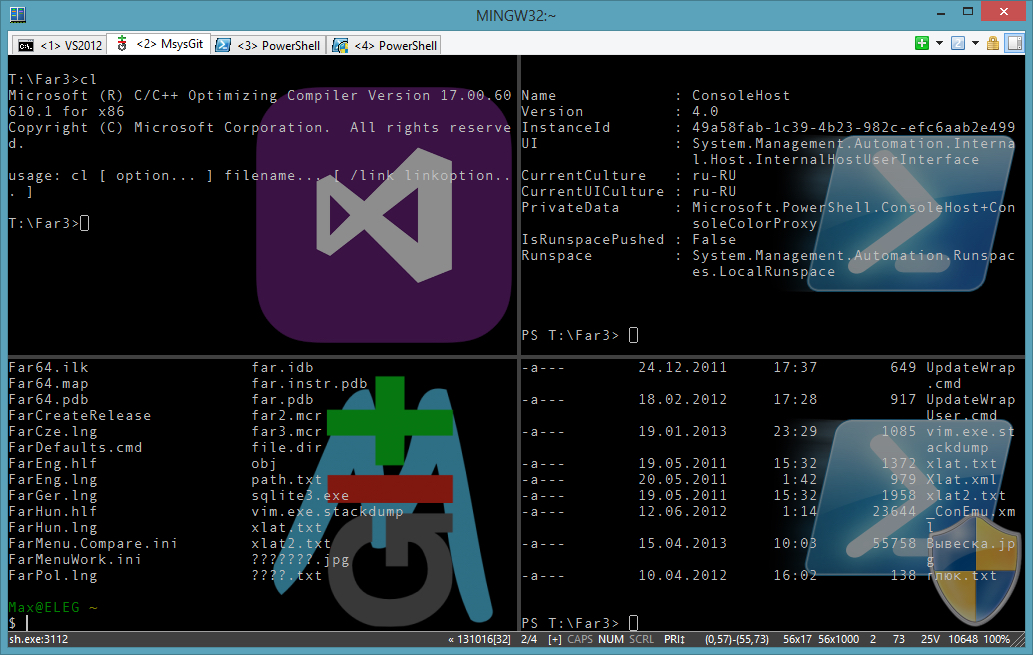
\includegraphics[scale=0.3]{img/conEmuImg.jpg}
\caption{Ukážka ConEmu emulátora}
\label{fig:test}
\end{figure}
\newpage
\subsubsection{cmder}
\indent Cmder je ďalším príkladom emulátora shell terminálu. Vychádza z troch projektov ConEmu, Clink a Git pre Windows - voľiteľná súčasť. ConEmu sme si predstavili v predcházajúcej časti s jeho kladymi a zápormi. Clink, konkrétne clink-completions je v projekte využívaný na zvýšenie komfortu pri písaní skriptov, nepridáva ďalšiu shellovú funkcionalitu. \cite{cmder}
\paragraph{Skúsenosti}
\indent ConEmu je príjemný nástroj, dokáže zjednodušíť človeku prácu obzvlášť ak je zvyknutý na programovanie v shell scripte. Nakoľko cmder používa ConEmu ako emulátor shell terminálu a je úzko určený pre Windows platformu nemožno hovoriť o multiplatformovom riešení.
\begin{figure}[!htbp]
	\centering
	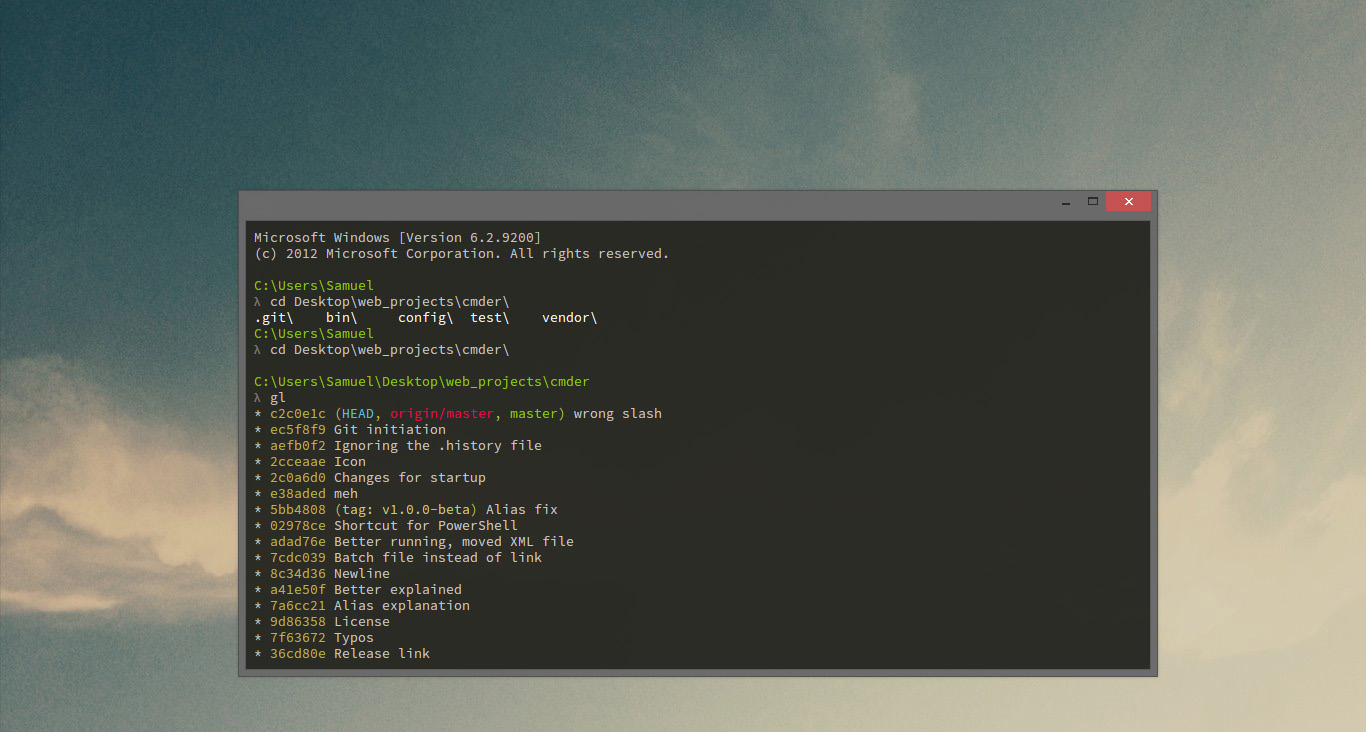
\includegraphics[scale=0.3]{img/cmder.jpg}
	\caption{Ukážka cmder emulátora}
	\label{fig:test}
\end{figure}
\newpage
\subsubsection{Babun}
\indent Babun je ďalším z množstva emulátorov pre Windows, ktorý je nadstavbou cygwinu. Vo svojom jadre používa zshell a bash, ktoré sme popísali ako populárne medzi komunitou. Prináľa vlasné gui, ktoré dokáže zafarbovať text podla zdrojoveho jazyka, čo zvyšuje prehľadnosť. Je tam git, svn, puython, perl. Tiež má integrované sťahovanie nových packagov, ktoré ponúka cygwin pomocou kľúčového slova pact. Prenositeľnosť skriptov z unixových strojov je zabezpečená tým, že používa bash a zsh, avšak je to emulátor čisto pre Windows distribúcie.\cite{babun}
\begin{figure}[!htbp]
	\centering
	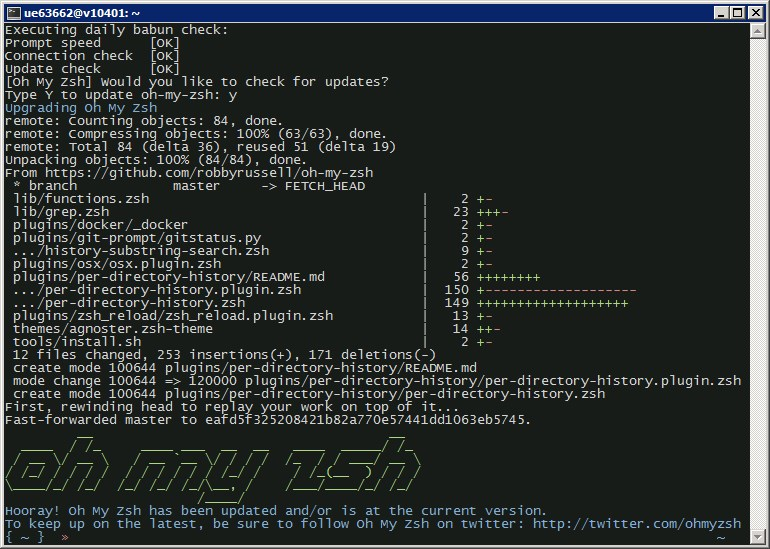
\includegraphics[scale=0.4]{img/babun.jpeg}
	\caption{Ukážka babun emulátora}
	\label{fig:test}
\end{figure}
\subsubsection{MobaXterm}
\indent Poskytuje množstvo funkcionality avšak je zatažený licenciou v hodnote 50 eur. \cite{mobaxterm}
\paragraph{Neplatená verzia}
\begin{itemize}
	\item Plná podpora SSH a X serveru
	\item Vzdialená plocha (RDP, VNC, Xdmcp)
	\item Vzdialený terminál (SSH, telnet, rlogin, Mosh)
	\item X11-Forwarding
	\item Automatický SFTP prehliadač
	\item Podpora pluginovt
	\item Možnosť inšalačnej alebo prenositeľnej verzie
	\item Plná dokumentácia
	\item Maximálne 12 spojení
	\item Maximálne 2 SSH tunely
	\item Maximálne 4 maká
	\item Maximálne 360 sekúnd pre Tftp, Nfs a Cron
\end{itemize}

\paragraph{Platená verzia}

\begin{itemize}
	\item Všetky vymoženosti z neplatenej verzie Home Edition +
	\item Možnosť upraviť svoju uvítaciu správu a logo
	\item Modifikovať profilový skript
	\item Odstrániť nechcené hry, šetriče obrazovky alebo nástroje
	\item Nelimitovaný počet spojení
	\item Nelimitovaný počet tunelov a makier
	\item Nelimitovaný čas behu pre sieťové daemony
	\item Podpora centrálneho hesla
	\item Profesionálny support
	\item Doživotné právo používania
\end{itemize}

\subsection{Zhodnotenie analyzovaných technológií}
\indent Analýza ukázala, že väčšinový podiel na trhu osobných počítačov ako aj serverov si delia medzi sebou Unix/Linux a Windows operačné systémy. Preto sme si analyzovali hlavne programovacie jazyky, ktoré sú obľúbené administrátormi daných jazykov. Tiež sme prešli rôzne dostupné riešenia problému univerzálnej konzoly, avšak ani jeden z produktov neposkytoval kompatibilitu na oboch alebo viacerých systémoch, nanjvyš kopíroval funkcie jedného systému do druhého. Na základe týchto poznatkov, ako aj poznatkov podrobnejšie rozpísaných v predchádzajúcich častiach sme sa rozhodli pokračovať v analýze prekladu jazykov a získané vedomosti pretaviť do vlastného univerzálneho platformovo nezávislého konzolového riešenia.

\section{Preklad jazykov}
\indent Pri programovacích jazykoch nás zaujímajú ich vyjadrovacie schopnosti ako aj vlastnosti z hľadiska ich rozpoznania. Tieto vlasnosti sa týkajú programovania a prekladu, pričom obe je potrebné zohľadniť pri tvorbe jazyka. V dnešnej dobe sa používajú na programovanie hlavne takzvané vyššie programovacie jazyky, môžeme ich označiť ako zdrojové jazyky. Na to aby vykonávali čo používateľ naprogramoval je potrebné aby boli pretransformované do jazyka daného stroja. Spomínanú transformáciu zabezpečuje prekladač, prekladačom máme na mysli program, ktorý číta zdrojový jazyk a transformuje ho do cieľového jazyka, ktorému rozumie stroj.\cite{gram}

\subsection{Kompilátor proces prekladu}
Aby bol preklad možný, musí byť zdrojový kód programu napísaný podľa určitých pravidiel, ktoré vyplývajú z jazyka. Proces prekladu je možné rodeliť na 4 hlavné časti.
\begin{itemize}
	\item lexikálna analýza
	\item syntakticka analýza
	\item spracovanie sémantiky
	\item generovanie cieľového jazyka
\end{itemize}
\indent Podrobnejšie si stručne popíšeme všetky štyri časti, ktoré majú pre nás z hľadiska prekladu najväčší zmysel.
\newline
\subsubsection{Lexikálna analýza}
	\indent Lexikálna analýza je prvou fázou kompilátora. Dopredu napísaný zdojový kód je postupne spracovávaný preprocesorom, ktorý vytvára takzvané lexémy. 
	 \newline Lexémou nazývame postupnosť alfanumerických znakov. Tieto postupnosti znakov sú následne vkladané do lexikálneho analyzátora, ktorý ma za úlohu vytvoriť zo vstupných lexém tokeny slúžiace ako vstup pre syntaktický analyzátor. 
	 \newline Tokeny sa vytvárajú na základe preddefinovaných pravidiel, ktoré sa v programovacích jazykoch definujú ako pattern. V prípade, že lexikálny analyátor nieje schopný nájsť  pattern pred danú lexému musí vyhlásiť chybu počas tokenizácie.  
	 \newline Výstupom z lexikálnej analýzy sú takzvané tokeny, ktoré tvoria vyššie jednotky jazyka ako kľúčové slová jazyka, konštanty, identifikátory, operátory a iné.\cite{gram}
	 
	 \begin{figure}[!htbp]
	 	\centering
	 	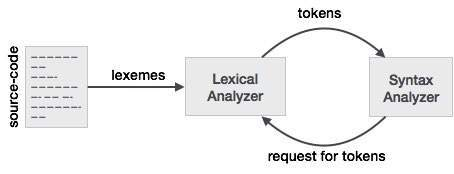
\includegraphics[width=15cm]{img/lexical_analysis.jpg}
	 	\caption{Ukážka práce lexikálneho analyzátora}
	 	\label{fig:test}
	 \end{figure}
 \newline
 
\subsubsection{Syntaktická analýza}
\indent Ďalšou fázou je syntaktická analýza. Úlohou Syntaktického analyzátora je kontrola správnosti vytvorených tokenov s uchovaním niektorých získaných informácií o štruktúre skúmanej syntaktickej jednotky. Syntaktická analýza sa radí medzi bezkontextové gramatiky. Po skoncení syntaktickej analýzy prichádza na rad sémantická analýza.\cite{gram}

 \newline
  \newline
\begin{figure}[!htbp]
	\centering
	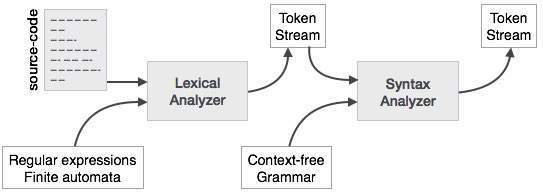
\includegraphics[width=15cm]{img/syntax_analyzer.jpg}
	\caption{Ukážka práce syntaktickeho  analyzátora}
	\label{fig:test}
\end{figure}
 \newline
 \newpage
\subsubsection{Limitácia syntaktickej analýzy}
\indent Syntaktický analyzátor ziska vstup z tokenu, ktorý vytvorí lexikálny analyzátor. Lexikálne analyzátory sú zodpovedné za validitu tokenu.Syntaktické analyzátory majú nasledovné limitácie.

\begin{itemize}
	\item nedokážu zistiť validitu tokenu
	\item nedokážu zistiť či je token používaný pred tým ako je deklarovaný
	\item nedokážu zistiť či je token používaný pred tým ako je inicializovaný
	\item nedokážu zistiť validitu operácie, ktorú token vykonáva
\end{itemize}



\subsubsection{Semantická  analýza}
\indent Sémantická analýza má za úlohu interpretovať symboly, typy, ich vzťahy.Sémantická analýza rohoduje či má syntax programy význam alebo nie.
Ako príklad zisťovania významu môžeme uviesť jednoduchú inicializáciu premennej.\cite{gram}

\begin{lstlisting}

	int integerVariable = 6

	int secondIntegerVariable = "six"
\end{lstlisting}

Oba príklady by mali prejsť cez lexikálnu a syntaktickú analýzu. Je až na sémantickej analýze aby rozhodla o správnosti zápisu programu a v prípade nesprávneho zápisu informovala o chybe.  Hlavné úlohy sémantickej analýzy sú" :

\begin{itemize}
	\item zisťovanie dosahu definovaných tokenov takzvaný scoping
	\item kontrola typov
	\item deklaracia premenných
	\item definícia premenných
	\item viacnásobná deklarácia premenných v jedno scope
\end{itemize}

\subsubsection{Generovanie cieľového jazyka}
\indent Generovanie cieľového jazyka môžeme považovať za poslednú fázu kompilátora. V tejto fáze sa preklápa jazyk z vyššieho jazyka do strojového jazyka, ktorý úspešne prešiel cez analyzačné časti .\cite{gram}

\subsection{Návrhové vzory}
\indent Návrhové vzory sú všeobecne opakovaným riešním pre všeobecne opakujúci sa problém pri dizajnovaní softwéru. Návrhový vzor nie je nemenný dizajn, vždy je potrebné aby si ho programátori uspôsobili podľa vlstných potrieb. Návrhové vzory sa delia do troch základných skupín vytváracie vzory, štrukturálne vzory a vzory správania. 

\subsubsection{Factory - továreň}
\indent Factory návrhový vzor patrí do sekcie vytváracích vzorov, pomocou tohoto vzoru budeme schopný vytvárať objekty bez toho aby sme prezradili logiku ich vytvárania klientovi.
Diagram návrhového vzoru je mozné vidieť na nasledujúcom obrázku.
\begin{figure}[!htbp]
	\centering
	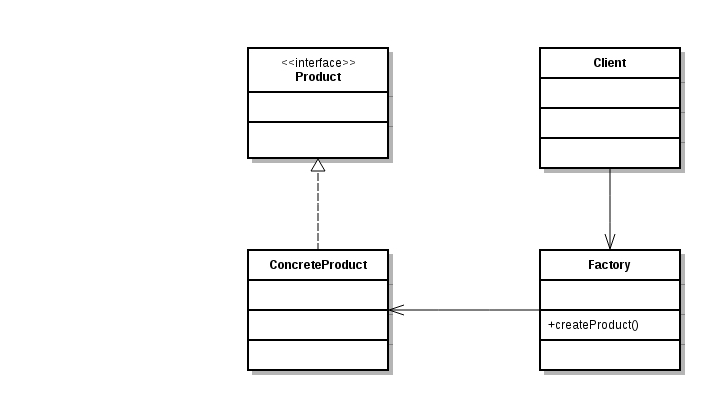
\includegraphics[width=10cm]{img/factory_design_pattern.jpg}
	\caption{Class diagram Factory návrhového vzoru}
	\label{fig:test}
\end{figure}
\newline
\subsubsection{Command - príkaz}
\indent Command pattern je známy behaviorálny návrhový vzor, používa sa najmä na menežovanie algoritmov, vzťahov a zodpovednosti medzi objektami. 
Cieľom vzoru je zapúzdriť požiadavku(request) ako objekt tým pádom parametrizovať klienta s rôznymi požiadavkami a zabezpečiť operáciu spať.
\begin{figure}[!htbp]
	\centering
	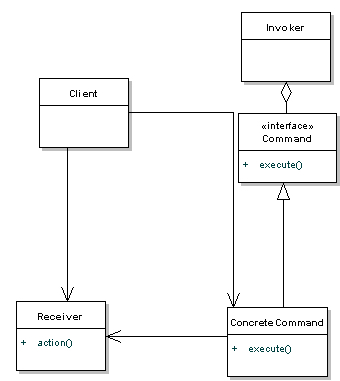
\includegraphics[width=10cm]{img/command_pattern_class.jpg}
	\caption{Class diagram Command návrhového vzoru}
	\label{fig:test}
\end{figure}
\newline
Command vzor deklaruje rozhranie pre všetky budúce commandy a zároveň execute() metódu, ktorú s vypýta Receiver commandu aby splnil požadovanú operáciu.
Receiver je objekt, ktorý vie ako požadovanú operáciu splniť. Invoker pozná command a pomocou implementovanej execute() metódy dokáže vyvolať požadovanú operáciu.
Klient potrebuje implemenotvaž ConcreteCommand a nastavit Receiver pre command. ConcreteCommand definuje spojenie medzi action a receiver. Keď Invoker zavolá execute() metódu na ConcreteCommand spustí tým jednu alebo viac akcií, ktoré budú bežať pomocou Receivera.

Pre lepšie pochopenie je proces zobrazený aj na sekvenčnom diagrame.
\begin{figure}[!htbp]
	\centering
	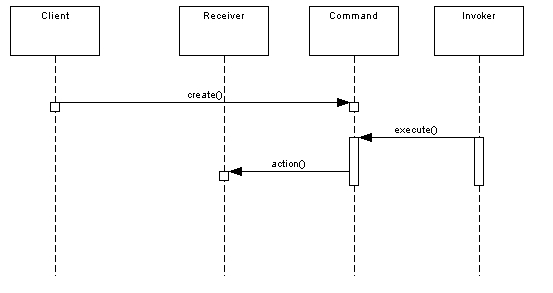
\includegraphics[width=10cm]{img/command_seq.jpg}
	\caption{Sekvenčný diagram Command návrhového vzoru}
	\label{fig:test}
\end{figure}
\newline

\section{Návrh riešenia}
\subsection{Prípady použitia}
\begin{figure}[!htbp]
	\centering
	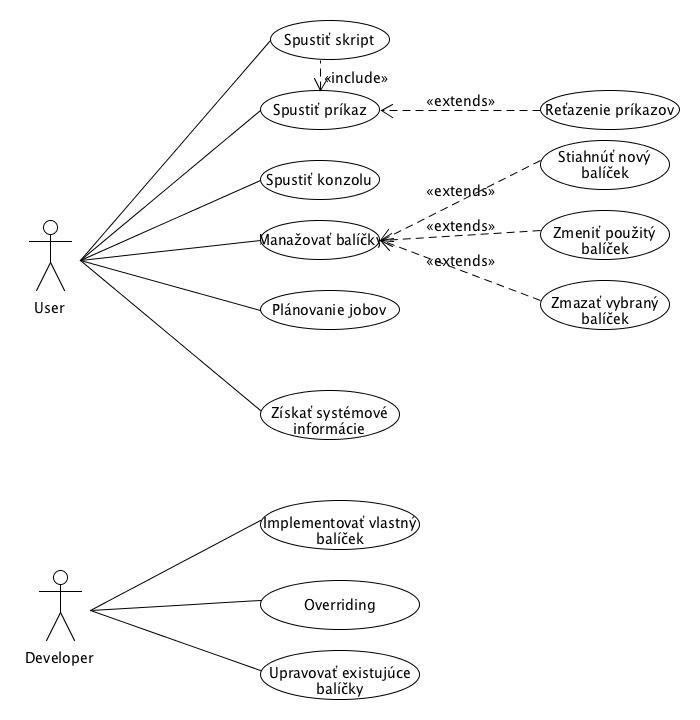
\includegraphics[width=\linewidth]{img/usecase.jpg}
	\caption{Prípady použitia pre navrhovanú aplikáciu}
	\label{fig:test}
\end{figure}
\newpage
\subsection{Popis prípadov použitia}
\indent V tejto časti sa venueme popisu jednotlivých use casov. Use case diagram spolu s popisom sú základnými prvkami na ktorých je možné špecifikovať novo vznikajúci softvér. Je dôležité aby najpodstatnejšie časti systému boli špecifikované na začiatku, aby sa pri navrhovaní aplikácie mohli prijať rozhodnutia, ktorými bude možné zaručiť, že výsledné riešenie bude to najlepšie možné, vyhovujúce špecifikácii. Ako je zjavné aj z priloženého diagramu prípadov použitia, pre aplikáciu sme identifikovali dvoch hráčov : Vývojár skriptov a Vývojár balíčkov. Títo hráči majú jednu spoločnú črtu - pre obe platí, že hráč je vývojár. Avšak je rozdiel medzi vývojárom skriptu a vývojom nových súčastí systému, čo je zjavne vidieť aj z popisu konkrétnych prípadov použitia.
\subsubsection{Vývojár skriptov}
\indent Rola sa zameriava hlavne na používanie hotovej aplikácie, prácu s balíčkami, vytváranie skriptov, efektívne využívanie dostupného \gls{api}. 
\paragraph{Spustiť konzolu}
\begin{center}
	\begin{longtable}{|p{2.5cm}|p{14cm}|}
		\hline
		\textbf{Use case} & Spustiť konzolu \\ 
		\hline
		\textbf{Podmienky} & Používateľ musí disponovať stiahnutou aplikáciou.\\
		\hline
		\textbf{Vstup} & Nie je potrebný žiany vstup od používateľa.\\
		\hline
		\textbf{Popis} & Konzolové rozhranie sa spustí. \\ 
		\hline
		\textbf{Výstp} & Konzola zobrazí základné údaje o konfigurácii.\\
		\hline
		\textbf{Chyba} & Konzola sa nespustí, musí však poskytnúť informáciu o chybe ktorá pri štarte nastala.\\
		\hline
	\caption{Use case : Spustiť konzolu}
	\label{table:1}
	\end{longtable}
\end{center}

\paragraph{Spustiť príkaz}
\begin{center}
	\begin{longtable}{|p{2.5cm}|p{14cm}|}
		\hline
		\textbf{Use case} & Spustiť príkaz \\ 
		\hline
		\textbf{Podmienky} & Shell aplikácia musí byť spustená \\ 
		\hline
		\textbf{Vstup} & Textový reťazec obsahujúci príkaz a jeho argumenty.\\
		\hline
		\textbf{Popis} & Používateľ zadá valídny príkaz, následne získa výstup pre zadaný príkaz. \\ 
		\hline
		\textbf{Výstp} & Textový reťazec, ktorý v závislosti od programu variuje v dľžke a obsahu.\\
		\hline
		\textbf{Chyba} & V prípade zlyhania je používateľ informovaný o probléme, ktorý nastal.\\
		\hline
		\caption{Use case : Spustiť príkaz}
		\label{table:1}
	\end{longtable}
	
\end{center}
\paragraph{Spustiť skript}
\begin{center}
	\begin{longtable}{|p{2.5cm}|p{14cm}|}
		\hline
		\textbf{Use case} & Spustiť skript \\ 
		\hline
		\textbf{Podmienky} & Shell aplikácia musí byť spustená a skript správne napísaný.\\ 
		\hline
		\textbf{Vstup} & Vstupom je skript, ktorý v hlavičke definuje balíčky ktoré bude používať. Za nimi môže nasledovať čokoľvek od definície premenných, funkcií. V tele skriptu musí byť zadefinovaná metóda main(String args).\\
		\hline
		\textbf{Popis} & Vykonajú sa všetky príkazy tak ako sú napísané v zdrojovom súbore. \\ 
		\hline
		\textbf{Výstp} & Výstup je textový reťazec, závislý na logike skriptu.\\
		\hline
		\textbf{Chyba} & V prípade chyby pri sťahovaní závislostí, exekúcie príkazov, alebo iných komplikácií za behu program zapisuje na stderr chybové hlášky spolu zo základným popisom problému, tracom.\\
		\hline
		\caption{Use case : Spustiť skript}
		\label{table:1}
	\end{longtable}

\end{center}

\paragraph{Spustiť shell príkaz}
\begin{center}
	\begin{longtable}{|p{2.5cm}|p{14cm}|}

			\hline
			\textbf{Use case} & Spustiť shell príkaz \\ 
			\hline
			\textbf{Podmienky} & Shell aplikácia musí byť spustená a skript správne napísaný. Taktiež musí byť v operačnom systéme ktorý podporuje shell. \\ 
			\hline
			\textbf{Vstup} & Textový reťazec obsahujúci príkaz a jeho argumenty.\\
			\hline
			\textbf{Popis} & Používateľ zadá valídny príkaz, následne získa výstup pre zadaný príkaz. \\ 
			\hline
			\textbf{Výstp} &Textový reťazec, ktorý v závislosti od programu variuje v dľžke a obsahu. \\
			\hline
			\textbf{Chyba} & V prípade zlyhania je používateľovi vratený chybový kód.\\
			\hline
		\caption{Use case : Spustiť shell príkaz}
	\label{table:1}
	
	\end{longtable}
\end{center}

\paragraph{Spustiť commander príkaz}
\begin{center}
	\begin{longtable}{|p{2.5cm}|p{14cm}|}

			\hline
			\textbf{Use case} & Spustiť commander príkaz \\ 
			\hline
			\textbf{Podmienky} & Shell aplikácia musí byť spustená a skript správne napísaný. Systém musí mať nainštalovaný windows commander.\\ 
			\hline
			\textbf{Vstup} & Textový reťazec obsahujúci príkaz a jeho argumenty.\\
			\hline
			\textbf{Popis} & Používateľ zadá valídny príkaz zacinajuci win alebo ext, následne získa výstup pre zadaný príkaz. \\ 
			\hline
			\textbf{Výstp} &Textový reťazec, ktorý v závislosti od programu variuje v dľžke a obsahu. \\
			\hline
			\textbf{Chyba} & V prípade zlyhania je používateľovi vratený chybový výstup z príkazového riadku.\\
			\hline
	\caption{Use case : Spustiť powershell príkaz}
	\label{table:1}

	\end{longtable}
\end{center}
\paragraph{Reťazie príkazov}
\begin{center}
	\begin{longtable}{|p{2.5cm}|p{14cm}|}

			\hline
			\textbf{Use case} & Reťazie príkazov \\ 
			\hline
			\textbf{Podmienky} & Shell aplikácia musí byť spustená. Vstup musí byť zadaný v správnom formáte.\\ 
			\hline
			\textbf{Vstup} & Textový reťazec obsahujúci sekvenciu príkazov, ich argumenty spojené znakom pajpy "|".\\
			\hline
			\textbf{Popis} & Systém rozozná, že ide o zreťazený príkaz a následne začne vykonávať príkazy v poradí v akom boli zadané. Jednotlivé príkazy odovzdajú svoje výstupy svojmu nasledovníkovy po úspešnom ukončení. Príkazy sa vykonávajú až kým nepríde na posledný príkaz v sekvencii, alebo ako počas behu príde pri niektorom z príkazov ku chybe. O chybe je používateľ oboznámený a chyba je zapísaná na štandardný chybový výstup. \\ 
			\hline

			\textbf{Výstp} & Textový reťazec, ktorý v závislosti od programu variuje v dľžke a obsahu, výstup bude vygenerovaný posledným príkazom sekvencie.\\
			\hline

			\textbf{Chyba} & O chybe je používateľ oboznámený a chyba je zapísaná na štandardný chybový výstup.\\
			\hline
	\caption{Use case : Reťazie príkazov}
	\label{table:1}

	\end{longtable}
\end{center}


\paragraph{Manažovať balíčky}
\begin{center}
	\begin{longtable}{|p{2.5cm}|p{14cm}|}

			\hline
			\textbf{Use case} & Manažovať balíčky \\ 
			\hline
			\textbf{Podmienky} & Shell aplikácia musí byť spustená.\\ 
			\hline
			\textbf{Vstup} & Textový reťazec obsahujúci príkaz "pkg" alebo aky si vyberem a jeho argumenty.\\
			\hline
			\textbf{Popis} & Používateľ bude schopný nahrať, zmazať, nahradiť vybraný balíček. \\ 
			\hline
			\textbf{Výstp} & Textový reťazec, ktorý v závislosti od programu variuje v dľžke a obsahu - možno bude informovať o šťahovacom procese.\\
			\hline
			\textbf{Chyba} & O chybe je používateľ oboznámený a chyba je zapísaná na štandardný chybový výstup v podobe stack tracu napr. .\\
			\hline
	\caption{Use case : Manažovať balíčky}
	\label{table:1}

	\end{longtable}
\end{center}
\paragraph{Stiahnúť nový balíček}
\begin{center}
	\begin{longtable}{|p{2.5cm}|p{14cm}|}
			\hline
			\textbf{Use case} & Stiahnúť nový balíček \\ 
			\hline
			\textbf{Podmienky} & Shell aplikácia musí byť spustená. Príkaz na stiahnutie balíčka musí byť správne zadaný.\\ 
			\hline
			\textbf{Vstup} & Textový reťazec obsahujúci príkaz "pkg download <názov balička>"\\
			\hline
			\textbf{Popis} & Program sa ako prvé pozrie do adresára balíčkov či už daný balíček nebol stiahnutý, ak nie stiahne nový balíček. V opačnom prípade medzi aktívne balíčky načíta používateľom zvolený balíček.\\ 
			\hline
			\textbf{Výstp} & Textový reťazec  informujúci o úspešnosti sťahovania. Pre jeho načítanie je potrebný reštart aplikácie.\\
			\hline

			\textbf{Chyba} & Vypíše chybu do stderr v prípade, že daný balíček na servery neexistuje, používateľ nemá internetové pripojenie.\\
			\hline
		\caption{Use case : Stiahnúť nový balíček}
		\label{table:1}
		
	\end{longtable}
\end{center}

\paragraph{Zmeniť  použiťý balíček}
\begin{center}
	\begin{longtable}{|p{2.5cm}|p{14cm}|}
		
			\hline
			\textbf{Use case} & Zmeniť  použiťý balíček \\ 
			\hline
			\textbf{Podmienky} & Shell aplikácia musí byť spustená. Príkaz na zmenenie používaného balíčka musí byť správne zadaný.\\ 
			\hline
			\textbf{Vstup} & Textový reťazec obsahujúci príkaz "pkg change <názov nahradzovaného balička> <názov nahradzujúceho balička>\\
			\hline
			\textbf{Popis} & Program zmení používaný balíček z aktuálne používaného na balíček vybratý používateľom. Táto voľba je aplikovateľná iba pre spravovanie verzií existujúcich balíčkov. V prípade, že nahradzujúci balíček nieje dostupný lokálne, používateľ bude vyzvaný stiahnúť daný balíček.\\ 
			\hline
			\textbf{Výstp} & Textový reťazec informujúci o úspešnosti výmeny, alebo informujúci o potrebe stiahnutia balíčka.\\
			\hline
			\textbf{Chyba} & V prípade ak príde počas zmeny balíčkov k chybe, bude zapísana na stderr.\\
			\hline
		\caption{Use case : Zmeniť  použiťý balíček}
		\label{table:1}
		
	\end{longtable}
\end{center}

\paragraph{Zmazať vybraný balíček}
\begin{center}
	\begin{longtable}{|p{2.5cm}|p{14cm}|}
		
			\hline
			\textbf{Use case} & Zmazať vybraný balíček \\ 
			\hline
			\textbf{Vstup} & Textový reťazec obsahujúci príkaz "pkg delete <názov balička>.\\
			\hline
			\textbf{Podmienky} & Shell aplikácia musí byť spustená. Príkaz na zmazanie vybraného balíčka musí byť správne zadaný.\\ 
			\hline
			\textbf{Popis} & Program zmaže používateľom vybraný balíček z aktívnych balíčkov a následne ho fyzicky zmaže z disku. \\
			\hline

			\textbf{Výstp} & Textový reťazec informujúci o úspešnosti zmazania zadaného balíka\\
			\hline
			\textbf{Chyba} & V prípade nesprávneho odstránenia balíčka z aktívnych alebo pri následnom mazaní zo súborového systému bude informácia o chybe presmerovaná na stderr.\\
			\hline
		\caption{Use case : Zmazať vybraný balíček}
		\label{table:1}
		
	\end{longtable}
\end{center}
\paragraph{Získať systémové informácie}
\begin{center}
	\begin{longtable}{|p{2.5cm}|p{14cm}|}
		
			\hline
			\textbf{Use case} & Získať systémové informácie \\ 
			\hline
			\textbf{Vstup} & Vstupom je textový reťazec "sysinfo".\\
			\hline
			\textbf{Podmienky} & Shell aplikácia musí byť spustená. Používateľ vloží valídny príkaz na vyžiadanie systémových informácií. \\ 
			\hline
			\textbf{Popis} & Program vypíše na štandardný výstup informácie o systémových informáciách ako napríklad využitie procesoru, využitie pamäte RAM, využitie oddielu swap, teplotu zariadení a podobné.\\ 
			\hline
					
			\textbf{Výstp} & Výstupom je textový reťazec, formátovaný do riadkov. Každému riadku prislúcha jedna informácia napr. CPU, ďalší riadok RAM atď.. V prípade viac jadrového procesora sa vypísu informácie o každom z jadier.  \\
			\hline
			\textbf{Chyba} & V prípade, že používateľ nemá právo na získanie informácií program vypíse dôvod priamo na stdout. Tak isto tam vypíše aj akékoľvek chyby ku ktorým môže prísť počas behu.\\
			\hline
		\caption{Use case : Získať systémové informácie}
		\label{table:1}
		
	\end{longtable}
\end{center}

\paragraph{Získať informácie o procesoch}
\begin{center}
	\begin{longtable}{|p{2.5cm}|p{14cm}|}
		
			\hline
			\textbf{Use case} & Získať informácie o procesoch \\ 
			\hline
			\textbf{Vstup} & Vstupom je textový reťazec "processes".\\
			\hline
			\textbf{Podmienky} & Shell aplikácia musí byť spustená. Používateľ vloží valídny príkaz na vyžiadanie informácií o procesoch. \\ 
			\hline

			\textbf{Popis} & Program vypíše na štandardný výstup informácie o bežiacich procesoch, používateľoch, ktorý tieto procesy spúšťajú, koľko procesoru, pamäte RAM pouýívajú.\\ 
			\hline

			\textbf{Výstp} & Výstupom je prehľadný výpis v podobe tabuľky, kde každý riadok zodpovedá jednému procesu. Nad jednotlivými hodnotami je hlavný riadok, ktorý popisuje o akú hodnotu ide.\\
			\hline
			\textbf{Chyba} & V prípade, že nieje možné získať informácie o procesoch je táto skutočnosť zobrazená na stdout a popis chyby sa presmeruje na stderr.\\
			\hline
		\caption{Use case : Získať informácie o procesoch}
		\label{table:1}
		
	\end{longtable}
\end{center}
\paragraph{Vytvoriť skript}
\begin{center}
	\begin{longtable}{|p{2.5cm}|p{14cm}|}
		
			\hline
			\textbf{Use case} & Vytvoriť skript \\ 
			\hline
			\textbf{Podmienky} & Používateľ musí mať prístup k akémukoľvek textovému editoru.  \\ 
			\hline
			\textbf{Vstup} & Vstupom musí byť správne napísaný skript. \\
			\hline
			\textbf{Popis} & Používateľ napíše skrip, ktorá bude prečítaný programom a vykonaný.\\ 
			\hline
			\textbf{Výstp} & Skrip vráti výstup zo svojho beho buď na štandardný výstup alebo do súbor podľa toho ako je naimplementovaný.\\
			\hline
			\textbf{Chyba} & V prípade, že príde k menšej chybe informácia bude zobrazená používateľovi, resp. presmerovaná do súboru.\\
			\hline
		\caption{Use case : Vytvoriť skript}
		\label{table:1}
		
	\end{longtable}
\end{center}
\paragraph{Vytvoriť funkciu}
\begin{center}
	\begin{longtable}{|p{2.5cm}|p{14cm}|}
		
			\hline
			\textbf{Use case} & Vytvoriť funkciu \\ 
			\hline
			\textbf{Podmienky} & Používateľ musí mať prístup k akémukoľvek textovému editoru.  \\ 
			\hline
			\textbf{Vstup} & Funkcia musí byť správne zadefinovaná. 
			Synax pre definovanie funkcie : 
			\newline
			function <návratový typ> <názov funkcie>(parametre funkcie){telo funkcie}. \\
			\hline
			
			\textbf{Popis} & Používateľ napíše funkciu, ktorá bude prečítaná programom a vykonaná.\\ 
			\hline

			\textbf{Výstp} & Funkcia vracia premennú s definovanou návratovou hodnotou.\\
			\hline
			\textbf{Chyba} & V prípade, že nastane chyba pri exekúcii funkcie program skončí a program zapíše informácie o chybe na stderr.\\
			\hline
		\caption{Use case : Vytvoriť funkciu}
		\label{table:1}
		
	\end{longtable}
\end{center}
\paragraph{Override funkcie}
\begin{center}
	\begin{longtable}{|p{2.5cm}|p{14cm}|}
		
			\hline
			\textbf{Use case} & Override funkcie \\ 
			\hline
			\textbf{Podmienky} & Používateľ musí mať prístup k akémukoľvek textovému editoru.  \\ 
			\hline
			\textbf{Vstup} & Nad funciou je potrebné zapísať @Override  čo prekladaču povie, že má používať práve túto verziu funkcie.\\
			\hline
			
			\textbf{Popis} & Používateľ napíše funkciu, ktorá bude prečítaná programom a vykonaná. Navyše bude nahradzovať funkciu s rovnakým názvom.\\ 
			\hline
			\textbf{Výstp} & Premenná, ktorá je uvedená v definícii funkcie.\\
			\hline
			\textbf{Chyba} & V prípade zle zadefinovanej syntaxe je problém zapísaný na stderr a vykonávanie skriptu je ukončené.\\
			\hline
		\caption{Use case : Override funkcie}
		\label{table:1}
		
	\end{longtable}
\end{center}
\paragraph{Vytvoriť cyklus}
\begin{center}
	\begin{longtable}{|p{2.5cm}|p{14cm}|}
		
			\hline
			\textbf{Use case} & Vytvoriť cyklus \\ 
			\hline
			\textbf{Podmienky} & Používateľ musí mať prístup k akémukoľvek textovému editoru.  \\ 
			\hline
			\textbf{Vstup} & Cyklus musí byť správne zadefinovaný. 
			Synax pre definovanie funkcie : 
			\newline
			for(<inicializácia premennej>;<podmienka pre spustenie>;<inkrement>){telo cyklu obsahujúce volania funkcií, príkazy, atď..}. \\
			\hline

			\textbf{Popis} & Používateľ napíše cyklus, ktorý bude prečítaný programom a vykonaná sa.\\ 
			\hline
			\textbf{Výstp} & Cyklus nemá žiadny výstup.\\
			\hline
			\textbf{Chyba} & V prípade, že nastane chyba pri parsovaní alebo exekúcii cyklu program skončí a program zapíše informácie o chybe na stderr.\\
			\hline
		\caption{Use case : Vytvoriť cyklus}
		\label{table:1}
		
	\end{longtable}
\end{center}
\paragraph{Vytvoriť podmienku}
\begin{center}
	\begin{longtable}{|p{2.5cm}|p{14cm}|}
		
			\hline
			\textbf{Use case} & Vytvoriť podmienku \\ 
			\hline
			\textbf{Podmienky} & Používateľ musí mať prístup k akémukoľvek textovému editoru.  \\ 
			\hline
			\textbf{Vstup} & Podmienka musí byť správne zadefinovaná. 
			Synax pre definovanie podmienky : 
			\newline
			if(boolean value){telo podmienky obsahujúce volania funkcií, príkazy, atď..}. \\
			\hline
			\textbf{Popis} & Používateľ napíše podmienku, ktorá bude prečítaná programom a zohľadnená za behu skriptu.\\ 
			\hline
			\textbf{Výstp} & Podmienka nemá žiadny výstup.\\
			\hline
			\textbf{Chyba} & V prípade, že nastane chyba pri parsovaní alebo exekúcii podmienky program skončí a program zapíše informácie o chybe na stderr.\\
			\hline
		\caption{Use case : Vytvoriť podmienku}
		\label{table:1}
		
	\end{longtable}
\end{center}
\paragraph{Vytvoriť premenné}
\begin{center}
	\begin{longtable}{|p{2.5cm}|p{14cm}|}
		
			\hline
			\textbf{Use case} & Vytvoriť premenné \\ 
			\hline
			\textbf{Podmienky} & Používateľ musí mať prístup k akémukoľvek textovému editoru.  \\ 
			\hline
			\textbf{Vstup} & Premenná musí byť správne zadefinovaná. 
			\newline
			Synax pre definovanie premennej : 
			\newline
			<typ> <názov premennej>; alebo 
			\newline
			 <typ> <názov premennej> = <hodnota>;
			 \newline
			 , kde hodnota môže byť konkrétna hodnota alebo iná premenná rovnakého typu.\\
			\hline
			\textbf{Popis} & Používateľ napíše inicializáciu alebo definíciu premennej, ktorá bude prečítaná programom a vykonaná.\\ 
			\hline
			\textbf{Výstp} & Program si uloží premmenú a jej hodnotu ak bola definovaná.\\
			\hline
			\textbf{Chyba} & V prípade, že nastane chyba používateľ bude informovaný o neúspechu na stderr.\\
			\hline
			\caption{Use case : Vytvoriť premenné}
		\label{table:1}
	
	\end{longtable}
\end{center}
\paragraph{Vykonať základné aritmetické operácie}
\begin{center}
	\begin{longtable}{|p{2.5cm}|p{14cm}|}
		
			\hline
			\textbf{Use case} & Vykonať základné aritmetické operácie \\ 
			\hline
			\textbf{Podmienky} & Používateľ musí mať prístup k akémukoľvek textovému editoru.  \\ 
			\hline
			\textbf{Vstup} & Premenná musí byť správne zadefinovaná. 
			\newline
			Synax pre definovanie /zmenu hodnoty premennej: 
			\newline
			<názov premennej> = <výraz>; alebo 
			\newline
			<typ> <názov premennej> = <výraz>;
			\newline
			, kde výraz môže byť operácia nad číselnými hodnotami a číselnými premennými. \\
			\hline
			\textbf{Popis} & Používateľ napíše príkaz, ktorá bude prečítaný programom a vykonaný.\\ 
			\hline
			\textbf{Výstp} & Príkaz nastaví hodnotu premennej s vypočítanou návratovou hodnotou.\\
			\hline
			\textbf{Chyba} & V prípade, že nastane chyba pri exekúcii príkazu program skončí a program zapíše informácie o chybe na stderr.\\
			\hline
		\caption{Use case : Vytvoriť funkciu}
		\label{table:1}
		
	\end{longtable}
\end{center}
\paragraph{Vykonať základné logické operácie}
\begin{center}
	\begin{longtable}{|p{2.5cm}|p{14cm}|}
		
			\hline
			\textbf{Use case} & Vykonať základné logické operácie\\ 
			\hline
			\textbf{Podmienky} & Používateľ musí mať prístup k akémukoľvek textovému editoru.  \\ 
			\hline
			\textbf{Vstup} & Premenná musí byť správne zadefinovaná. \newline
			Synax pre definovanie /zmenu hodnoty premennej:  \newline
			<názov premennej> = <výraz>; alebo \newline
			<typ> <názov premennej> = <výraz>;
			\newline
			, kde výraz môže byť operácia nad číselnými hodnotami , číselnými premennými ako aj nad pravdivostnými.\newline
			Vzťahy medzi číselnými hodnotami musia byť definované logickými operátormi - <, >, <=, >=, ==, !=.\newline
			Vzťahy medzi pravdivostnými hodnotami musia byť definované logickými operátormi : ==, !=, ||, \&\&.  \\
			\hline
			\textbf{Popis} & Používateľ napíše príkaz, ktorá bude prečítaný programom a vykonaný.\\ 
			\hline
			\textbf{Výstp} & Príkaz nastaví hodnotu premennej s vypočítanou návratovou hodnotou.\\
			\hline
			\textbf{Chyba} & V prípade, že nastane chyba pri exekúcii príkazu program skončí a program zapíše informácie o chybe na stderr.\\
			\hline
		\caption{Use case : Vytvoriť funkciu}
		\label{table:1}
		
	\end{longtable}
\end{center}

\paragraph{Presmerovať chybový výstup}
\begin{center}
	\begin{longtable}{|p{2.5cm}|p{14cm}|}
		
			\hline
			\textbf{Use case} & Presmerovať chybový výstup \\ 
			\hline
			\textbf{Vstup} & Pre presmerovanie na chybový výstup je potrebné dodržať syntax command stderr> file\\
			\hline
			\textbf{Podmienky} & Shell aplikácia musí byť spustená. Používateľ vloží valídny príkaz na presmerovanie chybového výstupu. \\ 
			\hline
			\textbf{Popis} & Program presmeruje chybový výstup kam mu používateľ v príkaze prikáže. \\ 
			\hline
			\textbf{Výstp} & Výstup programu predstavuje textový reťazec s popisom chyby, ktorá nastala.\\
			\hline
			\textbf{Chyba} & Ak by došlo k chybe zaloguje sa do logu aplikácie.\\
			\hline
		\caption{Use case : Presmerovať chybový výstup}
		\label{table:1}
		
	\end{longtable}
\end{center}
\paragraph{Presmerovať štandardný výstup}
\begin{center}
	\begin{longtable}{|p{2.5cm}|p{14cm}|}
		
			\hline
			\textbf{Use case} & Presmerovať štandardný výstup \\ 
			\hline
			\textbf{Podmienky} & Shell aplikácia musí byť spustená. Používateľ vloží valídny príkaz na presmerovanie štandardného výstupu. \\ 
			\hline
			\textbf{Vstup} & Pre presmerovanie na štandardný výstup je potrebné dodržať syntax command stderr> file\\
			\hline
			\textbf{Popis} & Program presmeruje štandardný výstup kam mu používateľ v príkaze prikáže.\\ 
			\hline
			\textbf{Výstp} & Výstup programu predstavuje textový reťazec s výstupom zo skriptu alebo príkazu.\\
			\hline
			\textbf{Chyba} & Ak by došlo k chybe zaloguje sa do logu aplikácie.\\
			\hline
		\caption{Use case : Presmerovať štandardný výstup }
		\label{table:1}
		
	\end{longtable}
\end{center}



\subsubsection{Vývojár balíčkov}
\indent Ako je z názvu role zjavné, tento hráč bude mať na starosti hlavne vývoj aplikácie, starať sa o jej funkcionalitim v zmysle rozširovania API, ktoré môže vývojár skriptov používať pre efektívnejšiu prácu.
\paragraph{Implementovať vlastný balíček}
\begin{center}
	\begin{longtable}{|p{2.5cm}|p{14cm}|}
		
			\hline
			\textbf{Use case} & Implementovať vlastný balíček \\ 
			\hline
			\textbf{Podmienky} & Používateľ musí mať nainštalovanú Java SDK vo verzii 8, mať prístup k textovému editoru.  \\ 
			\hline
			\textbf{Vstup} & Balíček obsahujúci všetky potrebné rozhrania, ktoré musí vývojár balíčka implementovať.\\
			\hline
			\textbf{Popis} & Používateľ implementuje novú funkcionalitu v jave, následne všetky zdrojové súbory skompiluje a pridá do jar súboru určeného na ukladanie nových balíčkov.\\ 
			\hline
			\textbf{Výstp} & Balíček, ktorý je možné nahrať do aplikácie a používať ako jeden z príkazov.\\
			\hline
			\textbf{Chyba} & Chyba môže nastať pri vytváraní balíčka, kedy ho o chybe informuje prekladač jazyka v ktorom je balíček implementovaný. V prípade neúspešného načítania je používateľ informovaný priamo v konzole na stout.\\
			\hline
		\caption{Use case : Implementovať vlastný balíček}
		\label{table:1}
		
	\end{longtable}
\end{center}

\paragraph{Upravovať existujúce balíčky}
\begin{center}
	\begin{longtable}{|p{2.5cm}|p{14cm}|}
		
			\hline
			\textbf{Use case} & Upravovať existujúce balíčky \\ 
			\hline
			\textbf{Podmienky} &  Používateľ musí mať nainštalovanú Java SDK vo verzii 8, mať prístup k textovému editoru.  \\ 
			\hline
			\textbf{Vstup} & Zdrojové súbory už existujúceho balíčka.\\
			\hline
			\textbf{Popis} & Používateľ upraví implementáciu alebo pridá novú funkcionalitu v jave, následne všetky zdrojové súbory skompiluje a pridá do jar súboru určeného na ukladanie nových balíčkov\\ 
			\hline
			\textbf{Výstp} & Po úprave je balíček možné nahrať do aplikácie a používať ako jeden z príkazov.\\
			\hline
			\textbf{Chyba} & \\
			\hline
		\caption{Use case : Upravovať existujúce balíčky}
		\label{table:1}
		
	\end{longtable}
\end{center}
\subsection{Java}
\indent Java je programovací jazyk a výpočtová platforma, ktorá bola vydaná spoločnosťou Sun Microsystems v roku 1995. \cite{java} 
Java je objektovo orientovaný jazyk - v Jave je všetko objekt, ktorý je možné jednoducho rozšíriť. Je platformovo nezávislá , kompiluje vstupný kód do byte kódu, ktorý nieje špecifický pre konkrétnu platformu, ale do kódu, ktorý dokáze spustiť \gls{jvm}. Vykompilovaný kód sa potom jednoducho spustí na pc v ktorom existuje \gls{jvm}. Jednoduchú na učenie, stačí poznať základy \gls{oop} a človek sa Javu rýchlo naučí. Bezpečná keďže obsahuje  bezpečnostné baláčky a funkcie pomocou, ktorých je možné vytvoriť bezpečné aplikácie. Samozrejmosťou pre javu je podpora paralelného spúštania procesov, ktoré následne bežia vo vláknach. Je považovaná za veľmi výkonnú a dynamickú.\cite{javatut}


\subsection{Aplikácia}
\indent Nakoľko sme sa rozhodli implementovať vlastné riešenie bolo potrebné zamyslieť sa a identifikovať na základe prípadov použitia z akých častí bude naša alikácia pozostávať. Keďže sme nechceli aby sme vytvorili jednu veľkú robustnú aplikáciu, ktorá by sa časom mohla a s najväčšou pravdepodobnosťou by sa  aj stala neudržiavateľnou. Nakoľko naše aplikácia musí byť schopná umožniť používateľom interaktívny a aj skrtiptovací módus. Rozhodli sme sa, že navrhneme jednu hlavnú aplikáciu, ktorá bude mať na starosti umožnovať interaktívny prístup pre používateľa ako aj skriptovací modus, no funkcionality, ktoré bude podporovať externalizujeme do menších podprogramov - pluginov, ktoré sa do apikácie budu nahrávať pri štarte. Aby sme mohli docieliť požadované výsledky rozhodli sme sa použiť, návrhový vzor Command. Ako ďalšie sme definovali komponenty aplikácie.

\subsection{Komponenty aplikácie}
\indent Po vybratí návrhového vzoru sme prešli na identifikáciu komponentov aplikácie. V prvom návrhu sme identifikovali niekoľko komponentov, ktoré považujeme za podstatné a potrebné pre správnych chod programu. Z týchto komponentov sme následne vytvorili malý projekt, kde sme sa pokúsili vytvoriť pár pluginov implementovaných pomocou command dizajnového návrhu na demonštrovanie funkčnosti. Nakoľko bol model funkčný rozhodli sme sa pokračovať s jeho vývojom. Uvádzame aj komponenty ktoré sme identifikovali pri vytváraní tejto ukázky funkčnosti.
\begin{itemize}
	\item Parser - vstupov aj vystupov
	\item Loader - na nahrávanie  jar súborov
	\item Sťahovač dependencií - jarka ktoré momentálne produkt neobsahuje napr. cusotm riešenia
	\item Scope - scope je oblasť kde sa definujú premenné, funkcie a pod. a tento komponent mal slúžiť na vytváranie scopov vrámci aplikácie.
	\item ScopeData - ktoré majú slúžiť na udržovanie dát v jednotlivých scopoch.
	\item ShellPlugin - komponent, ktorý nesie implementáciu príkazov.
\end{itemize}

 \begin{figure}[!htbp]
	\centering
	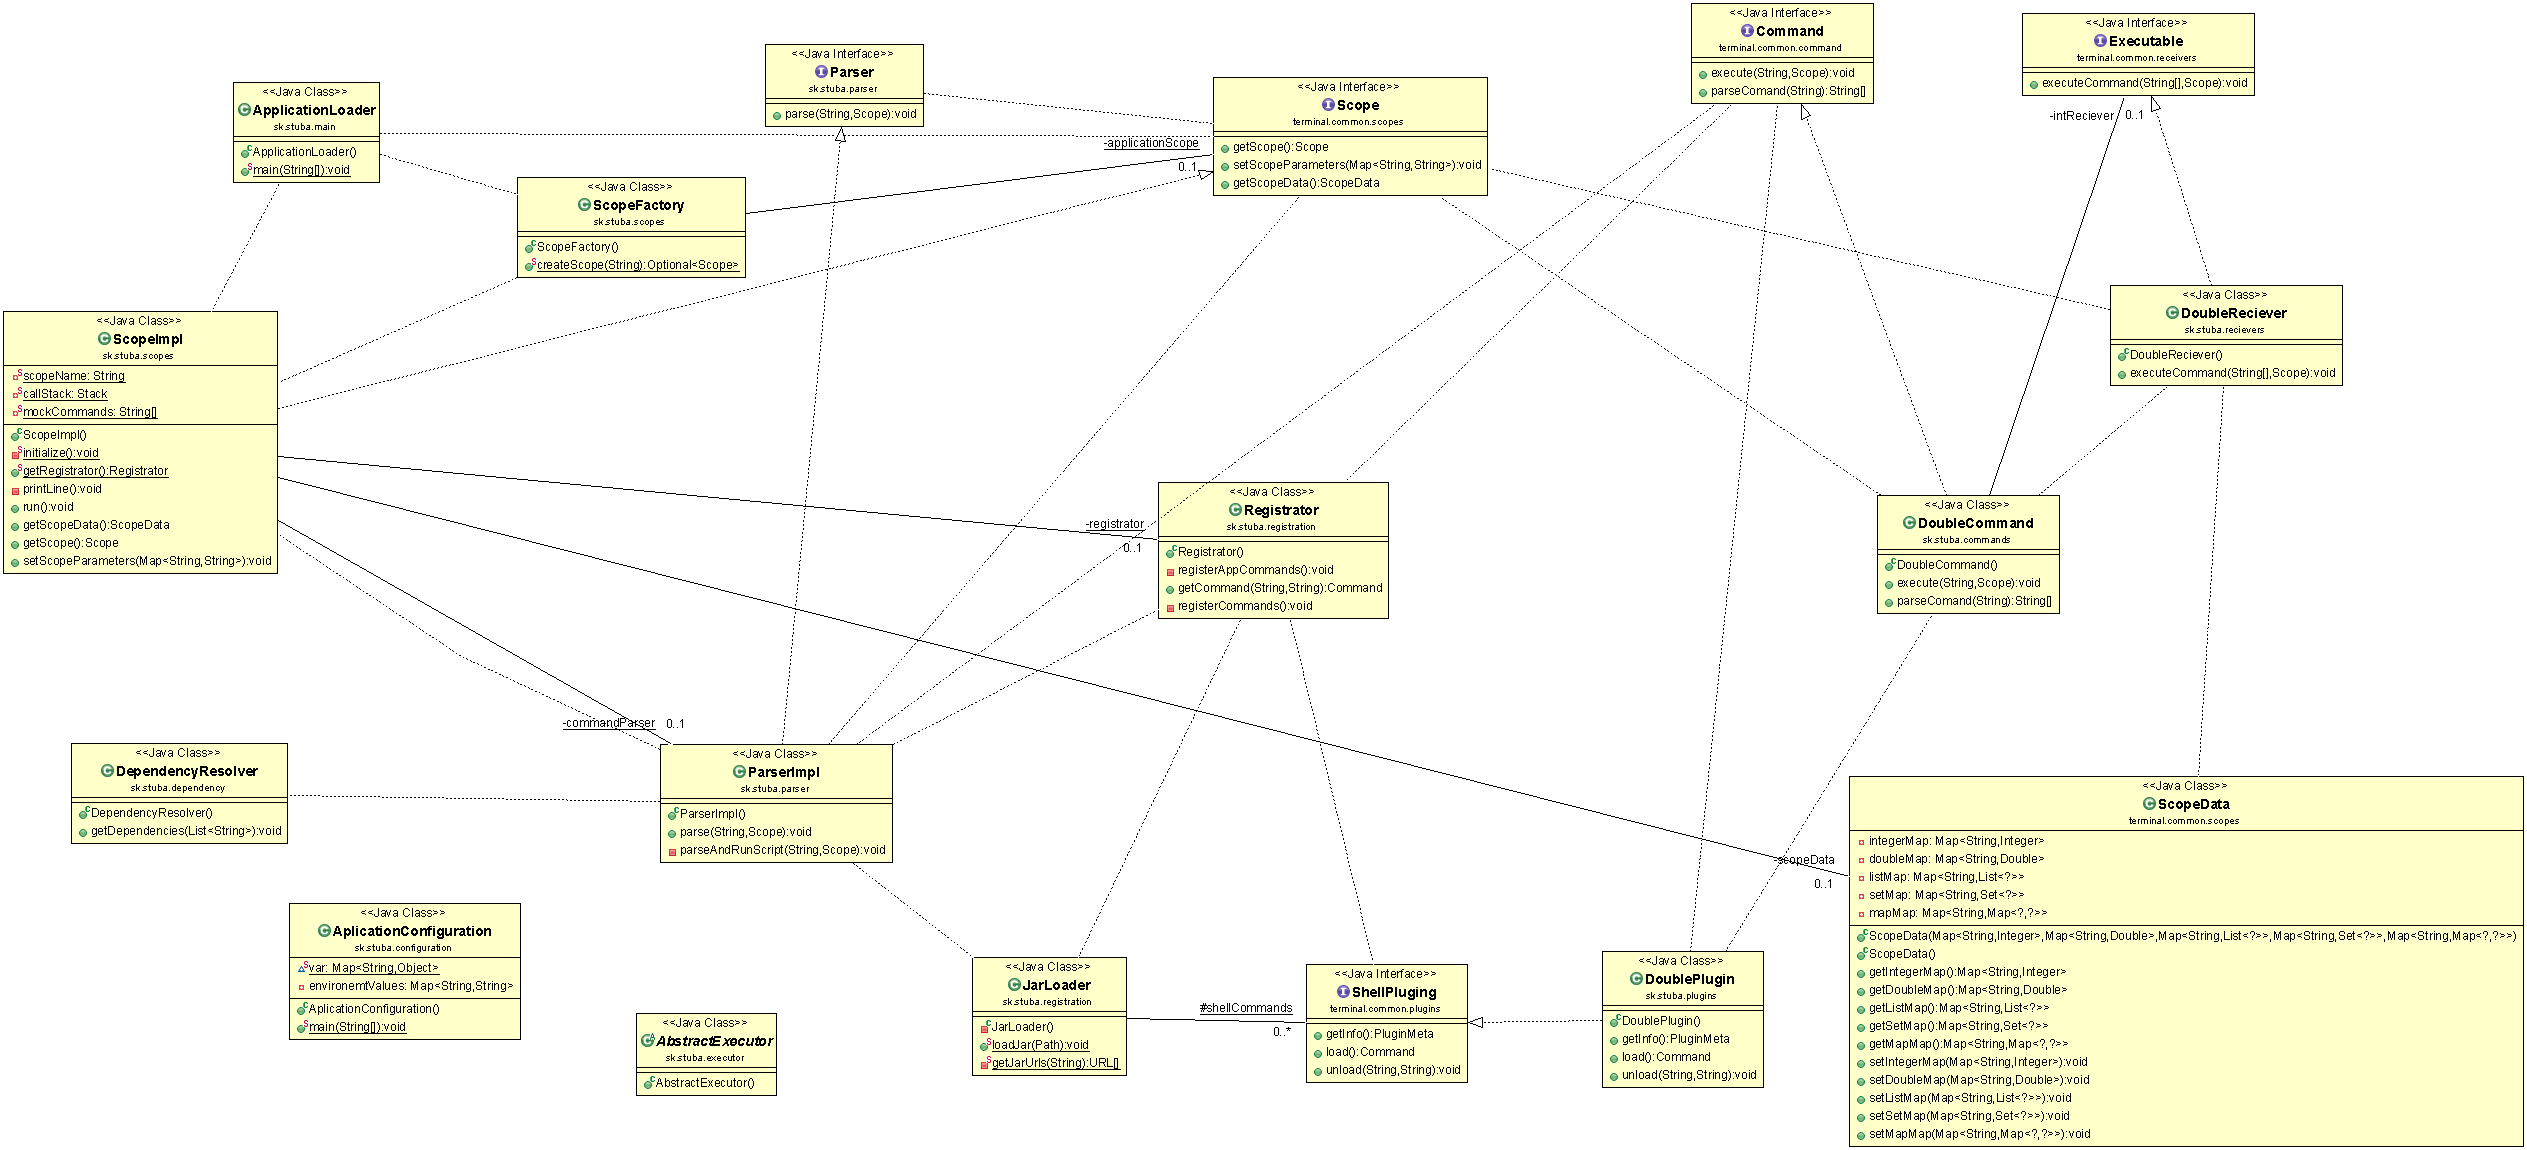
\includegraphics[width=\linewidth]{img/first_attemp_class_diag.jpg}
	\caption{Pvrvé funkčné riešenie}
	\label{fig:test}
\end{figure}
\newline
\subsection{Plugin}
\indent Z nasledovného class diagramu nebolo na prvý pohľad zreteľne viditeľné aké komponenty v programe existujú preto bolo potrebné zamyslieť sa ako by sa dali tieto časti rozumne rodeliť. Z prvotného návrhu sme vytiahli plugin, ktorý bude slúžiť na nahrávanie nových funkcionalít do programu.  Class diagram implementácie rozhraní a konkrétnych tried  je viditeľný na nasledovnom obrázku. 
 \begin{figure}[!htbp]
	\centering
	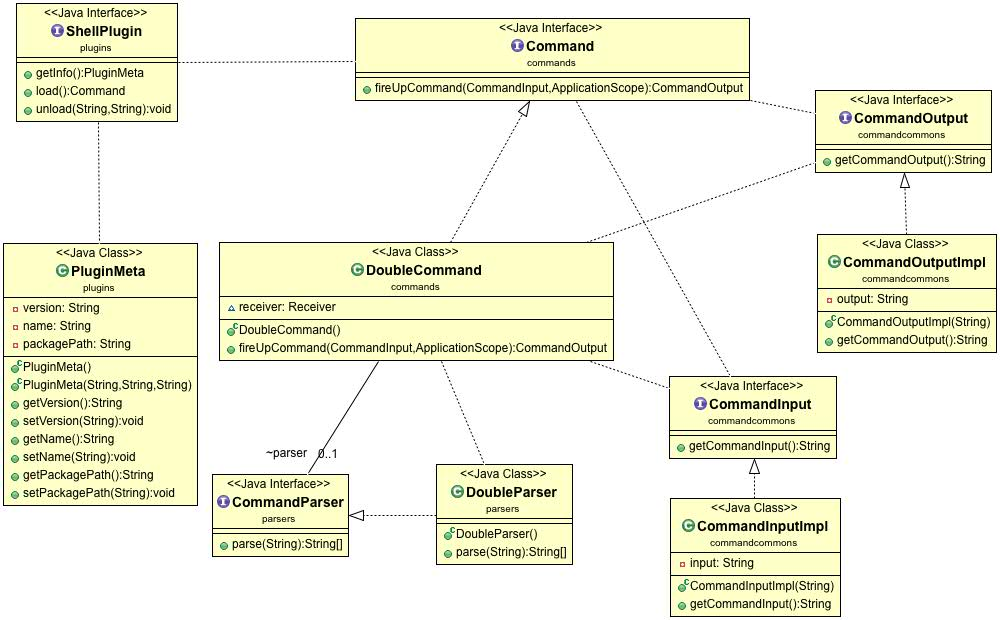
\includegraphics[width=\linewidth]{img/plugin_class.jpg}
	\caption{Class diagram pluginu}
	\label{fig:test}
\end{figure}
\newline
\indent Ako vidieť z diagramu Plugin pozostáva z nasledovných častí.
\begin{itemize}
	\item ShellPlugin - je rozhranie 
	\item Loader - na nahrávanie  jar súborov
	\item Sťahovač dependencií - jarka ktoré momentálne produkt neobsahuje napr. cusotm riešenia
	\item Scope - scope je oblasť kde sa definujú premenné, funkcie a pod. a tento komponent mal slúžiť na vytváranie scopov vrámci aplikácie.
	\item ScopeData - ktoré majú slúžiť na udržovanie dát v jednotlivých scopoch.
	\item ShellPlugin - komponent, ktorý nesie implementáciu príkazov.
\end{itemize}
Aj keď náš prvotý program fungoval správne čakali sme, že počas vývoja ešte môže dôjsť k obmenám tried a rozhraní, nakoľko málo kedy sa podarí odhadnúť  všetky kľúčové časti už počas návrhu.

\newpage
\subsection{Diagram tried aplikácie}
 \begin{figure}[!htbp]
	\centering
	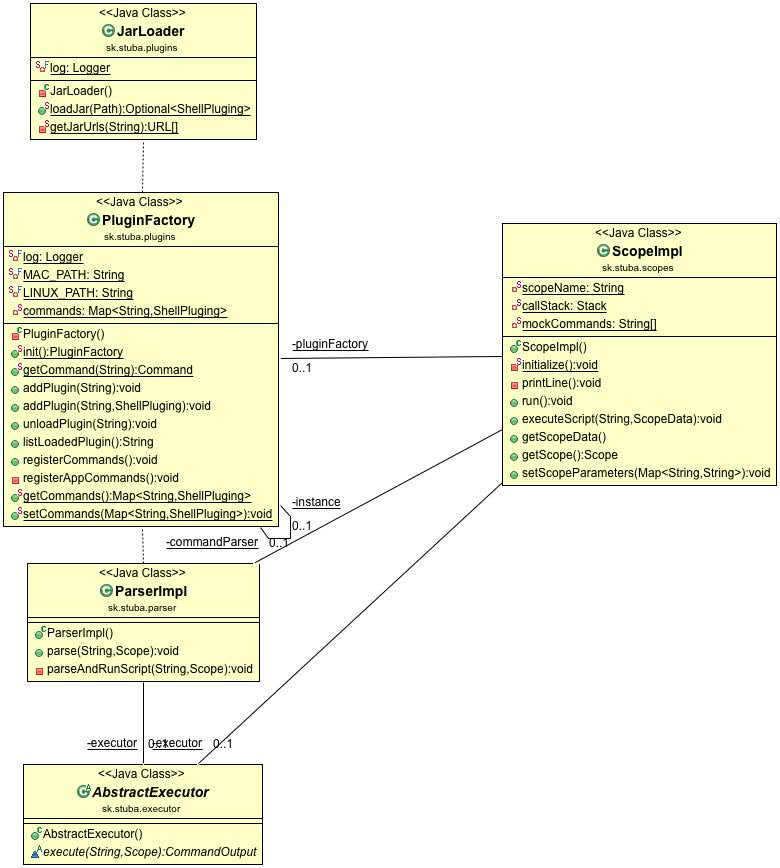
\includegraphics[scale=0.4]{img/ClassApplication.jpg}
	\caption{Diagram tried aplikácie}
	\label{fig:test}
\end{figure}
\subsubsection{Stručný popis tried}
\indent Obrázok 16 zobrazuje diagram tried aplikácie, ktoré su v nasledujúcej časti stručne predstavíme.
\paragraph{AbstractScope}
Táto trieda je jednou z najhlavnejších celého programu, tvorí základný pilier pre tvorbu akýchkoľvek scopov aplikácie, beh skriptov a pochopiteľne príkazov v interaktívnom móde. Nesie informácie o všetkých pluginoch, ktoré sa nahrali pri štarte aplikácie, názov scopu, exekútorovi pomocou ktorého sa vykonávajú všetky operácie v aplikácii. Trieda tiež nesie informácie o vstupných parametroch, výstupných hodnotách a funkciách, ktoré sú v danom scope definované. Spomenuté hodnoty sa využívajú pri vytváraní a behu skriptov. Implementuje rozhrania Scope, Runnable. Implementuje metódy run() pre zabezpečenie interaktívneho módu, kde sa však môžu spúšťať aj skripty. Tiež implementuje metódu executeScript(String function, ScopeVariables scopeVariables), slúži na rekurzívne volanie funkcií v skriptovacom móde a tiež  zbiehanie ich príkazov.
\paragraph{ScopeImpl}
Je prvá neabstraktná trieda, ktorá dedí od triedy AbstractScope, a slúži na inštanciáciu tejto triedy. 
\paragraph{ExecutorImpl}
Trieda ExecutorImpl implementuje rozhranie Executor a teda aj jeho triedu CommandIO execute(String command, Scope scope). Ako vstup do tejto metódy príde vstup od používateľa, a scope v ktorom ju chceme vykonať. Definovanie scopu nám slúži na informovanie jednotlivých prijímačov(Reciever) kde sa má daný príkaz vykonať. Ak by scope nebol presne definovaný aplikácia by sa nevedela rozhodnúť kde sa majú príkazy premietnuť.
\paragraph{RootParser}
RootParser je najpodstatnejšia trieda pre skriptovací mód. Má za úlohu načítať zdrojové súbory skriptu a následne spustiť exekúciu ak parsovanie prebehlo v poriadku.
\paragraph{PluginFactory}
PluginFactory ako z jej nýzvu vyplýva je to továreň do ktorej sa pri štarte aplikácie nahrávajú všetky pluginy, ktoré sú pre aplikáciu dotupné. Na záskavanie dostupných pluginov sa využíva trieda JarLoader. 
\paragraph{JarLoader}
Je trieda, ktorá pomocou class loadera nahráva nové pluginy do aplikácie.
\section{Implementácia}
\section{Zhodnotenie výsledkov}
Zatiaľ sa toho nespravilo hodne ale verím, že sa to tu cele zaplní.